\documentclass[12pt]{book}

\usepackage{setspace}
\usepackage{graphicx}
\usepackage{makeidx}
\usepackage{hyperref}
\usepackage{url}
\usepackage[T1]{fontenc}
\usepackage[utf8]{inputenc}
\usepackage{tikz}
\usepackage{amsthm}
\usepackage{amsmath}
\usepackage{makeidx}
\usetikzlibrary{shadows}

% format end of chapter excercises
\newtheoremstyle{exercise}
  {12pt}        % space above
  {12pt}        % space below
  {}            % body font
  {}            % indent amount
  {\bfseries}   % head font
  {}            % punctuation
  {12pt}        % head space
  {}            % custom head
\theoremstyle{exercise}
\newtheorem{exercise}{Exercise}[chapter]

\makeindex

% automatically index glossary terms
\newcommand{\term}[1]{%
\item[#1:]\index{#1}}

%%%%%% End preamble
\begin{document}

\newcommand{\thetitle}{Think CAD}
\newcommand{\thesubtitle}{TBD}
\newcommand{\theauthors}{Benjamin Smith}
\newcommand{\theversion}{0.0.0}
\newcommand*\keystroke[1]{%
  \tikz[baseline=(key.base)]
    \node[%
      draw,
      fill=white,
      drop shadow={shadow xshift=0.25ex,shadow yshift=-0.25ex,fill=black,opacity=0.75},
      rectangle,
      rounded corners=2pt,
      inner sep=1pt,
      line width=0.5pt,
      font=\scriptsize\sffamily
    ](key) {#1\strut}
  ;
}
\title{\thetitle}
\author{\theauthors}


% half title ---  ---  ---  ---  ---  ---  ---  ---  ---  ---  ---

\thispagestyle{empty}

\begin{flushright}
\vspace*{2.0in}

\begin{spacing}{3}
{\huge \thetitle}
\end{spacing}

\vspace{0.25in}

Version \theversion

\vfill

\end{flushright}

%%%%%% begin document

\chapter{Preface}
Computer-aided design (CAD) is a powerful tool for
spatial investigation and manipulation. Like many 
powerful tools, its usage can be broken down into
simple steps. I hope to take you through those steps
the right way the first time, so that you build good
habits from day one.

\section{Who is this book for?}
This book assumes no fore-knowledge of CAD or engineering
concepts. We'll start from square one. This book is for
individuals who want to manipulate 2-D and 3-D objects. 
User groups that may find this work useful are:

\begin{itemize}
\item Budding mechanical engineering students. Though I've spent
very little time in my engineering career as a designer,
I still CAD regularly.

\item Hobbyists and artists. I've used CAD to help churn through ideas on personal projects where pencil-on-paper
sketches would be sufficient but slow.

\item Parents who, due to the Covid-19 pandemic, can now
add ``teacher'' to their resume. I wish the lessons in
this book had been a part of my early schooling.
\end{itemize}

\section{Why am I writing this book?}

I'm writing this book because:
\begin{itemize}
\item I, like many, was taught to CAD through word of
mouth. I was blessed to have strong mentors, but I 
believe one can build a solid foundation with 
well-designed lessons. Surprisingly, the resource I
envision doesn't seem to exist.

\item Instruction tends toward details, advanced theory,
and excess talk while missing fundamental concepts and,
most important, practice. I aim to create a book that,
like a good coach,
encourages practice, critical thought, and strong
fundamentals.

\item I believe that learning the skills well from 
Day 1 can shorten the learning curve by months. Learning
them haphazardly can build poor habits that later need to
be remodeled.

\item I've consumed my fair share of do-it-yourself
books. I hope to give back to that collection of knowledge.
\end{itemize}

\section{Using this Book}
This book is intended as a series of work-along exercises.
CAD, like most cognitive skills, is best learned with a
bit of listening and a lot of doing. I recommend these
steps to make the most of this book.

\begin{description}
\item[Mouse] Get yourself a mouse with at least two
buttons and a scroll wheel. I use one with a cord.
\item[This Book] Keep this book open as you work. This is
not a ``read-a-chapter-then-do'' type of book.
\item[Monitors] If you've got two monitors, great! I
don't. Find a way to easily view both Onshape and this book, preferably at the same time.
\end{description}

\section{Using Onshape}
This book uses Onshape because it
is free (as in beer), and therefore accessible. You
will need to make an account at (\url{onshape.com}).
Onshape's free accounts include storage space for public 
documents, which means other users can view and copy 
but not edit your documents. Onshape's free subscription
is not the place to develop highly confidential designs.
Perhaps the world needs less highly confidential designs.

\section{CAD Efficiency}
I find the following allow me to smoothly develop and manipulate my models. I recommend building these habits, and only shunning them once you've determined they don't work for you.

\begin{description}
\item[Hotkeys] I'll call out relevant hotkeys when appropriate. Because keystrokes are more practiced and require less precision than mouse clicks, they are faster for repetitive tasks such as defining a sketch. Where a hotkey appears as (\keystroke{shift} \keystroke{s}), this is translated as ``While holding \keystroke{shift}, press \keystroke{s}''.
\end{description}

\chapter{Hello World}

\section{The Workspace and Planes}
The default Onshape workspace contains three planes and
and an origin, shown in Figure \ref{chap01_planes}. The workspace is a virtual representation
of three-dimensional (3-D) space.

\begin{figure}[ht!]
\centerline{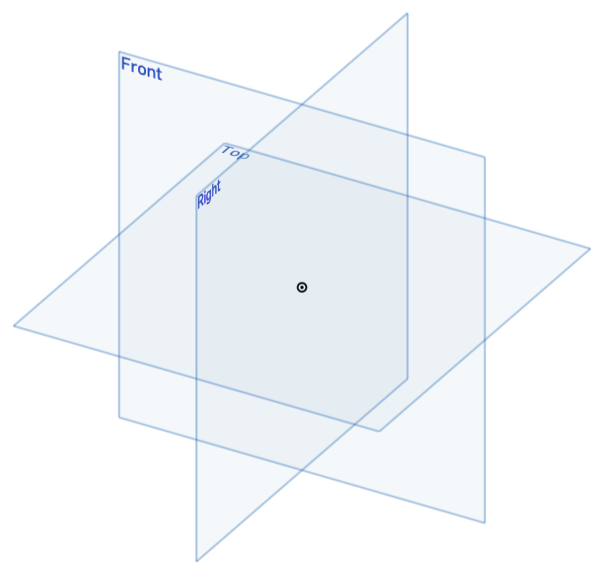
\includegraphics[width=5in]{figs/chap01_planes.png}}
\caption{Default planes intersecting at the origin.}
\label{chap01_planes}
\end{figure}

Planes are two-dimensional (2-D) slices through 3-D
space. All new parts in Onshape, like most CAD platforms
have the three planes, Top, Right, and Front. These
three planes are orthogonal, forming right angles
with each other and intersecting at the origin.

With the exception of motion simulations, gravity has no role in part development. This means that the Top, Right,and Front planes are equivalent, and parts can be developed in any orientation. All 2-D sketches must exist on a plane.

\index{planes}

\section{Moving and Selecting}
You can manipulate the workspace using the following 
mouse commands:

\begin{description}
\item[Zoom] with the scroll wheel.
\item[Rotate] by clicking the right mouse button and moving.
\item[Pan] by clicking the scroll wheel and moving.
Alternatively, you can hold 
\end{description}

Select a feature by clicking on it. Onshape uses persistent seletion, meaning that when you click on a second item, the first item remains selected, as in Figure \ref{chap01_selection}. The cursor tells you that two items are selected, and the {\bf feature tree} highlights which items those are. Deselect a single item by clicking it again. Deselect all items with the \keystroke{spacebar} or by clicking into empty space.

\begin{figure}[ht!]
\centerline{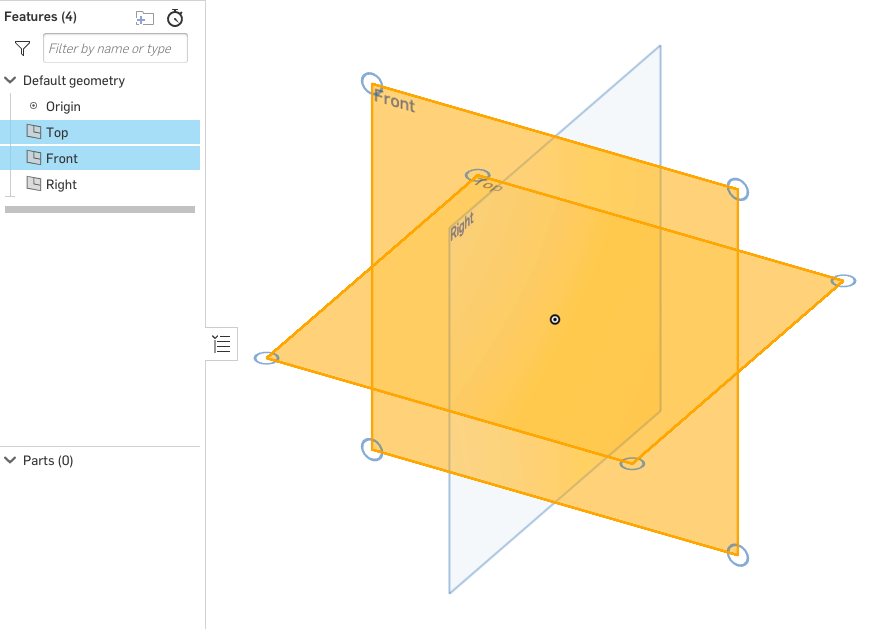
\includegraphics[width=5in]{figs/chap01_selection.png}}
\caption{Select multiple items by clicking on each. The feature tree (left) indicates which items are selected.}
\label{chap01_selection}
\end{figure}

\section{Sketches, Features, \& Models}
{\bf Sketches} provide two-dimensional geometry that act as the building block for three-dimensional parts. All sketches live on a plane. 

{\bf Features} turn two-dimensional sketches into three-dimensional solids and, less frequently, surfaces. Features often modify existing solids through Boolean operations such as addition, subtraction, or intersection.

{\bf Models}, also called parts, are the accumulation of three-dimensional features. Most models are {\bf solid models}, meaning that all features have thickness.
In contrast, {\bf surface models} have sketches and features but zero thickness. Like solid bodies, they are also the combination of multiple features.

Because sketches define two of the three dimensions of a feature, sketches capture the more detailed profile, and features extend that profile through space. If you were to CAD your hand, you might start with a sketch outlining your five fingers and palm, like the child's art project. Selecting the proper sketch profile builds a strong foundation for the rest of your model.

\section{The First Part}
As there is no traditional \href{https://en.wikipedia.org/wiki/%22Hello,_World!%22_program}{Hello World}
CAD part, I've elected that we'll make a triangular prism.

Start by selecting a single plane. Choose ``Sketch'' from the Feature Toolbar (\keystroke{shift} \keystroke{s}) to begin your sketch on that plane. 

It is often easier to sketch while viewing directly at, or normal to the plane. You can change your view by clicking on the View Cube, <right-click>-``View normal to'', or \keystroke{n}. I also prefer to toggle plane visibility off with the eyeball.

\begin{figure}[ht!]
\centerline{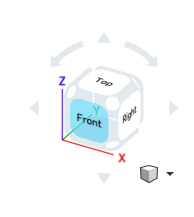
\includegraphics[width=3in]{figs/chap01_view_cube.png}}
\caption{The View Cube allows you to view models from pre-defined views.}
\label{view_cube}
\end{figure}

Sketch a right triangle with one leg vertical and one leg horizontal, both meeting at the origin, as in Figure \ref{start_sketch}. The two legs of the triangle are now black, meaning that they are {\bf constrained}. This means they are fully defined, and if you try to drag them, they will not move.

\begin{figure}[ht!]
\centerline{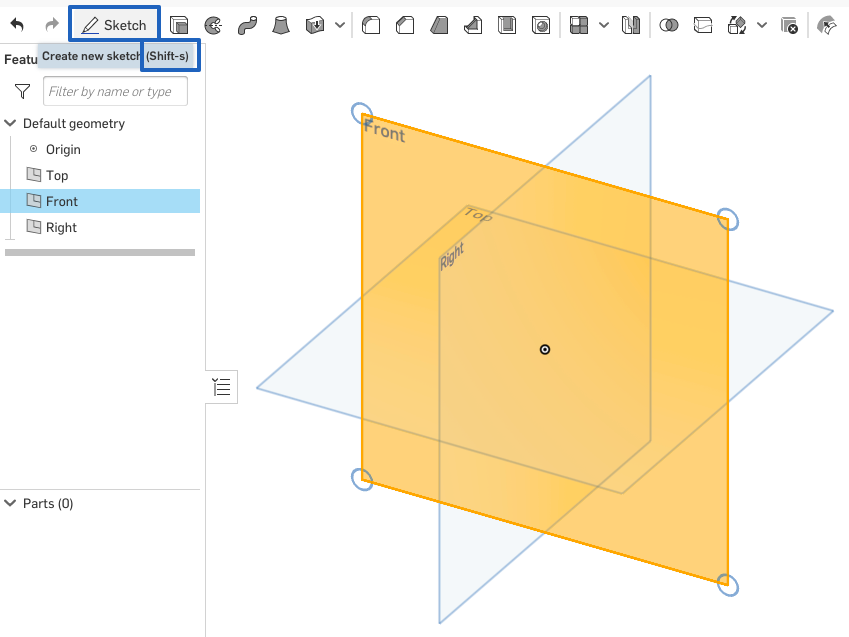
\includegraphics[width=4in]{figs/chap01_start_sketch.png}}
\caption{}
\label{}
\end{figure}

Note that the hypotenuse and each of its endpoints are blue, indicating that they are {\bf underconstrained}. Notice that endpoints move differently from edges when dragged. As sketches increase in complexity, it can be challenging to determine which degrees of freedom remain undefined. Dragging blue sketch entities can help you to understand where constraints are needed.

Constrain the sketch by adding a dimension (\keystroke{d}) of to one of the legs. Often, we'll want two dimensions to share the same size. We could accomplish this in a few ways.

\begin{description}
\item[Dimension both] - This is not preferable because changing
\end{description}

\section{Design Intent}
A key feature of well-done CAD is that it captures {\bf design intent}.

\section{Exercises}
\begin{exercise}
Locate the Onshape documentation on the extrude feature. Review the documentation for the desktop platform. Is it easier to access this documentation from the Onshape Help menu or from a search engine?
This will also be your first introduction to the Onshape mobile platforms, which won't be covered in this book.
\end{exercise}

\begin{exercise}
Modify your part to test additional options within Extrude. You might try these:

\begin{itemize}
\item Create a second closed shape within your triangle and extrude the first shape, second shape, both, or regions where they intersect.

\item Create a sketch on one of the faces of the first part. Extrude that sketch into or away from the prism, or in both directions. Test the ``New'', ``Add'', ``Remove'', and ``Intersect'' features. With each test, observe how many parts result in the Parts Tree.

\end{itemize}
\end{exercise}

\begin{exercise}
Delete constraints in your sketch until the sketch is underconstrained. Which ways are you able to move the sketch? Now constrain the sketch in different types of triangles, such as an equilateral. Can you make an isoceles triangle with a height that is twice the length of the base? Without equations?
\end{exercise}

\begin{exercise}
Change the first extrude to a surface rather than a solid. What happens when you try to add a solid body to a surface? What happens when you try to measure the thickness of one of the surfaces?
\end{exercise}


\end{document}
